\chapter{Studi Literatur}

Pada bab ini akan dideskripsikan kajian literatur yang terkait dengan persoalan Tugas Akhir. Studi literatur ini akan dijadikan dasar didalam melakukan penyelesaian persoalan yang telah didefinisikan.

\section{\textit{Spreadsheet}}
Bagian ini akan membahas mengenai definisi umum \textit{spreadsheet} serta teknologi yang sering digunakan didalam membuat \textit{spreadsheet}. Dengan adanya definisi umum ini diharapkan dapat menyamakan persepsi mengenai \textit{spreadsheet} yang dimaksud pada Tugas Akhir ini. Teknologi yang dijelaskan pada bagian ini merupakan teknologi yang memungkinkan untuk dijadikan dasar pengembangan perangkat lunak pada Tugas Akhir ini.

\subsection{Definisi Umum}
Secara harafiah, \textit{spreadsheet} adalah suatu perangkat lunak yang dapat melakukan kalkulasi terhadap angka serta mengorganisir informasi yang ada di dalamnya berdasarkan kolom dan baris \citep{meriamwebster-spreadsheet}. Konsep dasar pada aplikasi \textit{spreadsheet} modern adalah sebuah aplikasi yang berupa sekumpulan sel terdiri dari baris dan kolom yang disebut \textit{sheet} yang dapat digambarkan sebagai matriks yang besar \citep{Ronen1989}.

Sel-sel pada \textit{spreadsheet} dapat diisi data berupa data mentah maupun formula. Data mentah dapat berupa angka, teks, tanggal, dan nilai mata uang. Formula merupakan perintah yang dapat dimengerti komputer untuk menghitung dan memanipulasi data pada sel. Data hasil pengolahan dan masukan pada \textit{spreadsheet} ditampilkan dalam bentuk sel yang namanya terdiri dari nama kolom dan nilai baris (Contoh: A1 untuk kolom pertama dan baris pertama). Selain itu, sel tersebut juga dapat memiliki \textit{properties} berupa \textit{value} yang diisikan, format sel, serta format data yang digunakan.

\subsection{Teknologi \textit{Spreadsheet}} \label{TeknologiSpreadsheet}
Perkembangan teknologi \textit{spreadsheet} digital modern dimulai pada tahun 1978, saat Bricklin mengembangkan \textit{working prototype} dari konsep dasar \textit{spreadsheet} menggunakan Integer BASIC. Pada tahun yang sama, Frankston dan Fylstra bergabung dan membentuk sebuah perangkat lunak bernama VisiCalc (Visible Calculator) yang merupakan sebuah perangkat lunak \textit{spreadsheet} pertama yang bekerja dengan baik dan sukses dipasaran. Setelah keberhasilan VisiCalc, mulai muncul aplikasi serupa yang semakin baik salah satunya adalah Lotus. Dengan berkembangnya daya komputasi dan munculnya konsep \textit{graphical user interface}, Microsoft mengembangkan Microsoft Excel yang merupakan \textit{spreadsheet} pertama yang menggunakan antarmuka grafis dan menggunakan \textit{mouse} sebagai alat kontrol \citep{power2004brief}.

Saat ini, perangkat lunak berupa \textit{spreadsheet} sangat banyak variasi dan tipenya. Perangkat lunak \textit{spreadsheet} ini dapat dibagi berdasarkan konektivitasnya yakni \textit{offline spreadsheet} dan \textit{online spreadsheet}. Selain itu, perangkat lunak \textit{spreadsheet} dapat juga dibagi berdasarkan keterbukaan dari \textit{source code} yakni \textit{open source} dan \textit{closed source}. Bagian ini akan membahas masing-masing perangkat lunak tersebut secara umum.

    \subsubsection{Microsoft Excel}
    Microsoft Excel adalah perangkat lunak yang dikembangkan oleh Microsoft yang menyediakan fitur dasar dari \textit{spreadsheet} serta dengan fitur-fitur lainnya yang selalu ditambahkan pada setiap iterasi pengembangan Excel. Microsoft Excel dapat dimiliki oleh pengguna melalui pembelian paket Microsoft Office yang berisikan produk esensial Microsoft lainnya \citep{MSExcelProduct}. 

    Sejak Microsoft Excel 2007, Microsoft menggunakan format Office Open XML (OOXML) sebagai format penyimpanan \citep{MSExcelSupport}. Office Open XML dikembangkan oleh Microsoft mulai dari tahun 2000 dengan diimplementasinya dukungan XML pada Microsoft Office 2000. Pada awal penggunaan aplikasi \textit{office}, terdapat permasalahan \textit{data interoperability} antar mesin dan sulitnya manipulasi data. Office Open XML diharapkan dapat menyelesaikan permasalahan ini dengan membentuk standar yang dapat diimplementasi berbagai aplikasi \textit{office} \citep{OOXMLFormat}.

    \subsubsection{LibreOffice Calc}
    LibreOffice adalah perangkat lunak yang dikembangkan oleh komunitas dan proyek dari organisasi non-profit bernama The Document Foundation. LibreOffice adalah perangkat lunak yang gratis dan \textit{open source} yang awalnya didasarkan pada perangkat lunak serupa yakni OpenOffice.org dan merupakan pengembangan lanjutan dari OpenOffice yang paling aktif. Hampir serupa dengan Microsoft Office, LibreOffice memberikan 6 perangkat lunak yang ada di dalamnya yakni: Writer (pemrosesan teks), Calc (\textit{spreadsheet}), Impress (presentasi), Draw (grafik dan vektor), Base (basisdata), dan Math (editor formula) \citep{LibreOffice}. 

    LibreOffice Calc memiliki berbagai kemampuan yang dimiliki oleh kebanyakan \textit{spreadsheet}. Didalam melakukan penyimpanan file, Calc menggunakan format OpenDocument. Format OpenDocument dikembangkan oleh Organization for the Advancement of Structured Information Standards (OASIS) yang bertujuan untuk membentuk \textit{open standard} bagi \textit{office document} \citep{OpenDocument}. 

    \subsubsection{EtherCalc}
    EtherCalc merupakan perangkat lunak \textit{spreadsheet online} yang \textit{open-source} yang dikembangkan oleh Audrey Tang. EtherCalc merupakan pengembangan yang didasarkan dari perangkat lunak serupa yakni WikiCalc dan SocialCalc. WikiCalc merupakan aplikasi \textit{spreadsheet} yang mengandalkan komputasi server untuk dapat berkolaborasi, sedangkan SocialCalc merupakan aplikasi \textit{spreadsheet} yang menggunakan kemampuan javascript untuk melakukan komputasi pada \textit{client-side}. EtherCalc dikembangkan diatas Node.js dan menggunakan javascript sebagai alat komputasi. Perangkat lunak hanya akan melakukan panggilan ke \textit{server} saat melakukan suatu aksi dan \textit{server} yang bertugas untuk menyimpan kumpulan aksi tersebut agar pengguna lain yang ikut berkolaborasi dapat melihat \textit{spreadsheet} yang sama satu dengan yang lain \citep{EtherCalc}. Gambar \ref{IlustrasiEtherCalc} merupakan gambaran umum cara kerja EtherCalc dalam berkolaborasi.

    \begin{figure}[htb]
        \centering
        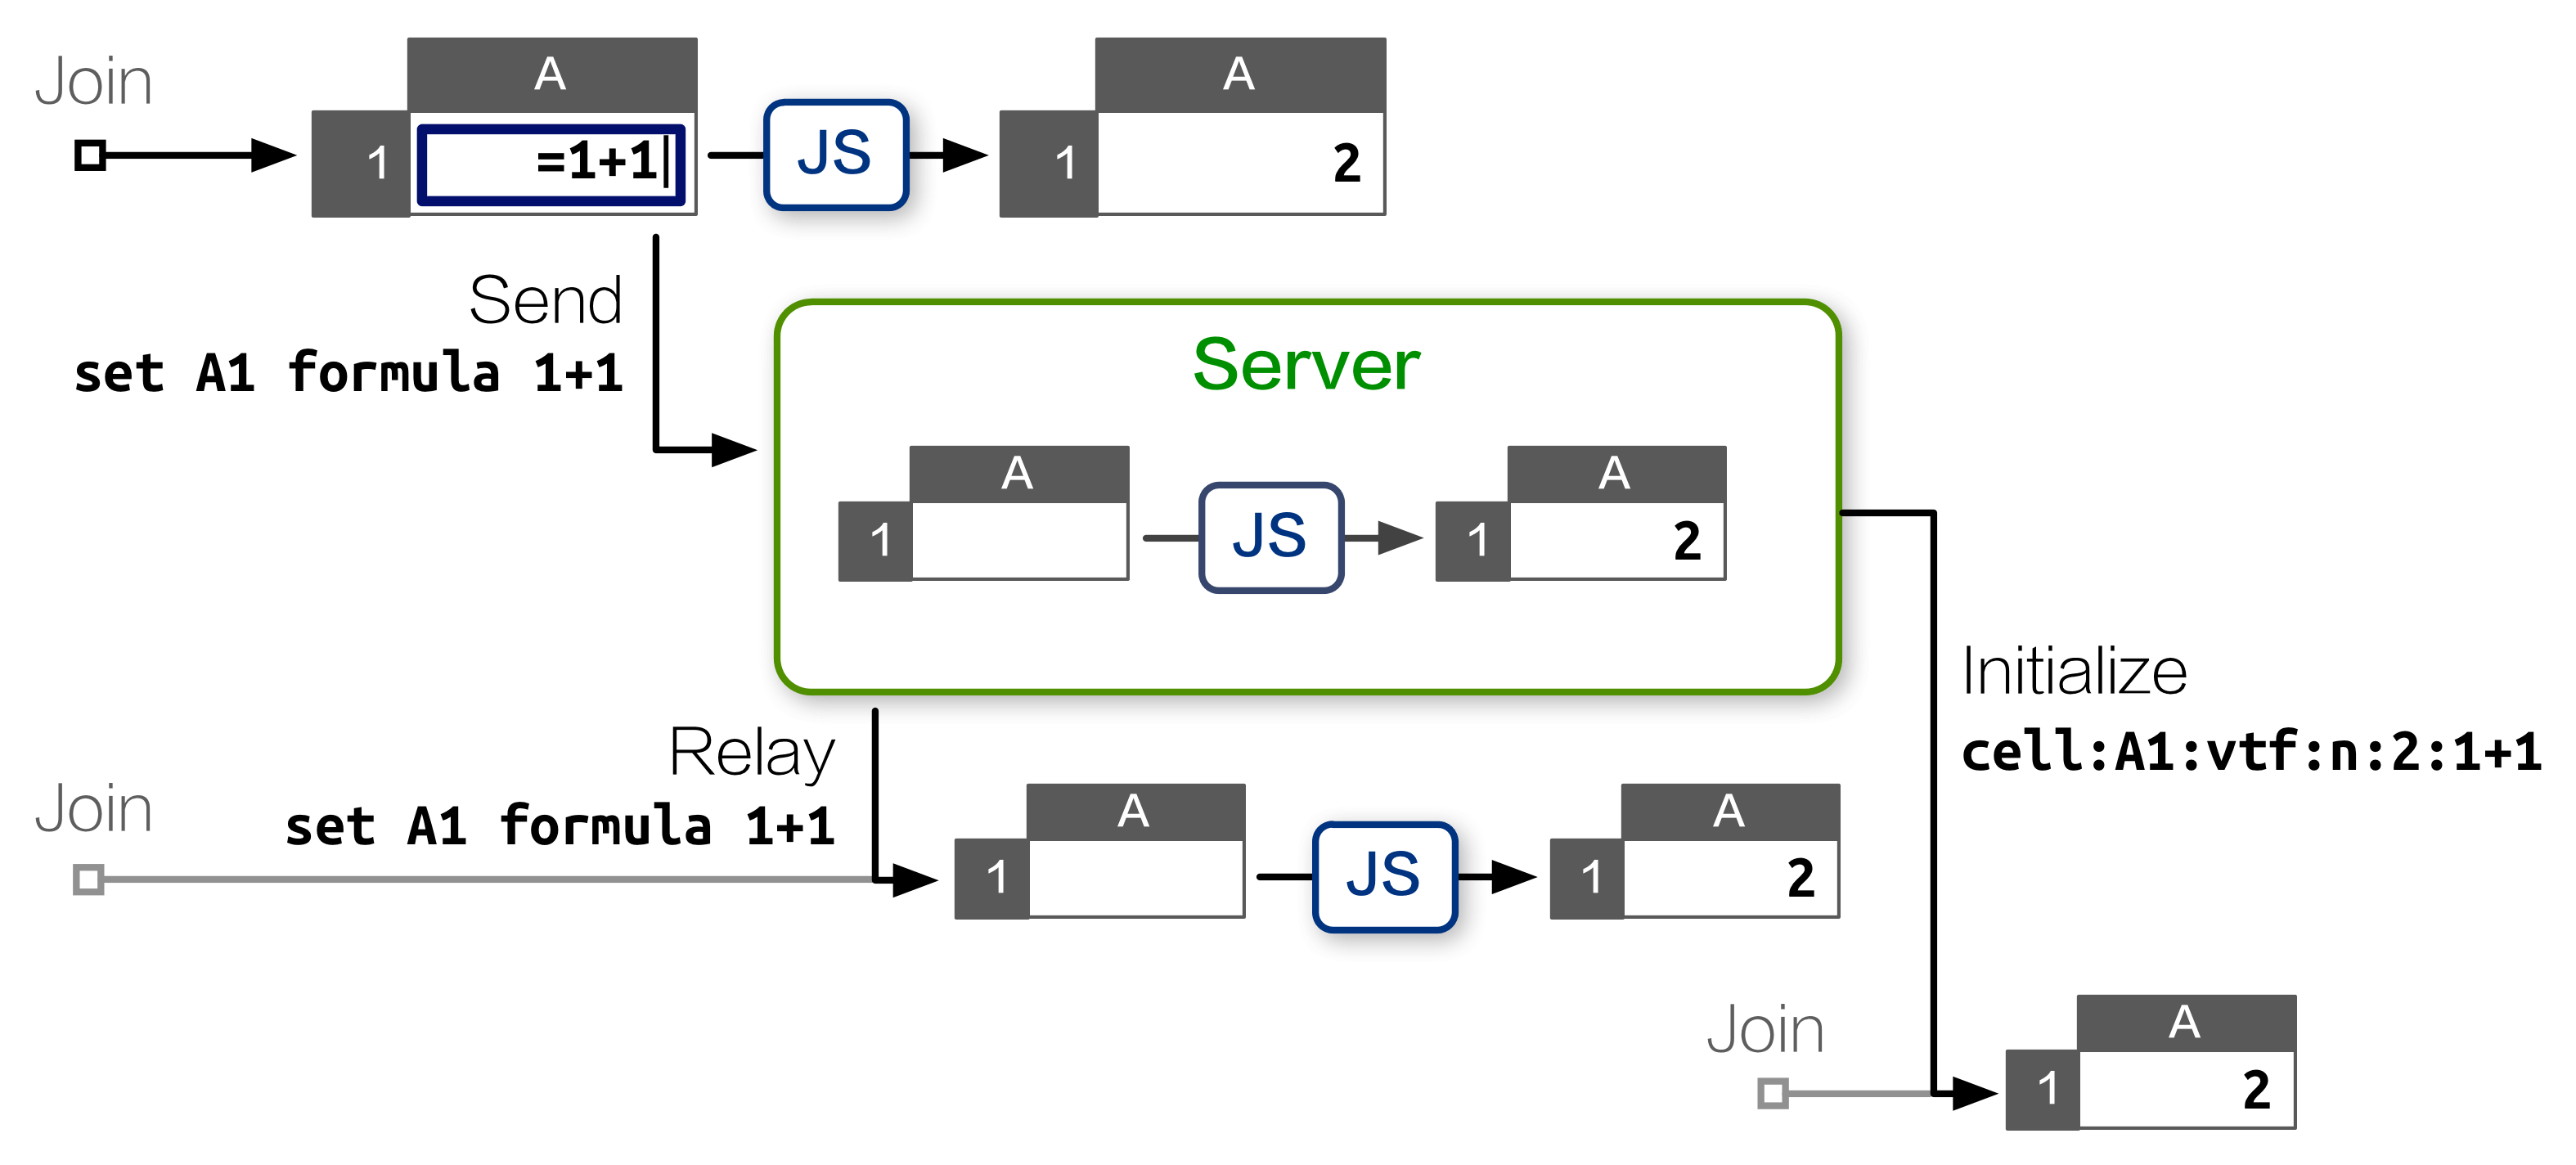
\includegraphics[width=0.6\textwidth]{resources/chapter-2-ethercalc.png}
        \caption{Ilustrasi Cara Kerja Kolaborasi pada EtherCalc}
        \label{IlustrasiEtherCalc}
    \end{figure}

    \subsubsection{Google Sheet}
    Google Sheet merupakan salah satu perangkat lunak pada \textit{office suite} miliki Google. Google Sheet dapat berjalan diatas tiga \textit{platform} yang berbeda yakni: sebagai \textit{web application}, Chrome apps, dan \textit{mobile apps}. Sheet memiliki kemampuan berkolaborasi secara \textit{real-time} dan menyediakan fitur-fitur \textit{spreadsheet} yang ada pada umumnya. Sheet memiliki fitur \textit{revision history} sehingga setiap orang dapat melihat perubahan yang terjadi, \textit{add-ons} yang dapat menambahkan fitur kepada Sheet melalui program yang dibuat oleh komunitas serta fitur \textit{chat} dengan kolaborator. Google Sheet dikembangkan menggunakan bahasa \textit{javascript} yang memberikan kemampuan penyimpanan dan kolaborasi secara \textit{real-time} \citep{GoogleSheet}.

    \subsubsection{OnlyOffice}
    Merupakan perangkat lunak sebagai \textit{service} yang dikembangkan oleh Ascensio System SIA. OnlyOffice merupakan \textit{office suite} yang berjalan diatas \textit{web application} yang dipadukan dengan sistem \textit{customer relationship management}. OnlyOffice tidak hanya terdiri dari \textit{online office editor} namun juga terdapat fitur managemen dokumen, manajemen proyek, \textit{mail service}, serta manajemen pelanggan seperti kontak, \textit{invoice}, \textit{opportonities}, dan \textit{task}. OnlyOffice ditujukan kepada bisnis yang membutuhkan perangkat lunak yang dapat mengorganisir kebutuhan bisnis didalam satu aplikasi yang saling terintegrasi \citep{OnlyOffice}. 


\section{Penggunaan \textit{Spreadsheet}}
\textit{Spreadsheet} dapat digunakan untuk melakukan kalkulasi terhadap suatu rumus atau formula yang sulit jika dikalkulasikan dengan cara manual. Selain itu, \textit{spreadsheet} dapat juga digunakan untuk melakukan ramalan terhadap suatu perubahan variabel masukan. Pada perkembangannya, \textit{spreadsheet} memiliki fitur-fitur tambahan seperti visualisasi data dan ekstraksi data penting dari kumpulan data yang ada.

Penelitian tentang penggunaan \textit{spreadsheet} pada bisnis pernah dilakukan sebelumnya pada tahun 2014. Subjek yang diteliti adalah akuntan manajemen \citep{Bradbard2014}. Pada penelitian tersebut, didapatkan gambaran umum mengenai penggunaan \textit{spreadsheet} secara umum. Menurut hasil penelitian tersebut beberapa fitur yang sering digunakan oleh pengguna \textit{spreadsheet} secara terurut dari yang paling sering digunakan adalah sebagai berikut,

\begin{enumerate}
    \item Menghitung fungsi matematika dasar (tambah, kurang, kali, bagi, dan lainnya)
    \item Mengelola \textit{worksheet} dan \textit{workbook} (menambahkan, menghapus, merubah nama, dan lainnya)
    \item Melakukan perubahan format dasar (menebalkan, memberi garis bawah, format angkat, dan lainnya)
    \item Melakukan pengurutan data, penghitungan subtotal, serta meringkas data
    \item Menggunakan fitur \textit{cell addressing} baik absolut maupun relatif
    \item Penggunaan fungsi kondisi (IF, COUNTIF), fungsi logika (AND, OR), fungsi pencarian (VLOOKUP, HLOOKUP), menautkan \textit{workbook} lain, serta fungsi pembulatan (ROUND, CEILING, FLOOR)
\end{enumerate}

Penggunaan \textit{spreadsheet} sangat bergantung kepada domain bisnis atau organisasi yang menggunakan. Pada bisnis yang berorientasi komersial, \textit{spreadsheet} dapat digunakan sebagai alat bantu perhitungan laba, pengeluaran, investasi, dan pajak. Pada organisasi-organisasi non komersial, \textit{spreadsheet} dapat digunakan sebagai salah satu bentuk basis data yang menangani penyimpanan, pengelolaan, dan pengumpulan data yang mudah dan cepat.

\section{Kesalahan dalam Penggunaan \textit{Spreadsheet}}
\subsection{Kualitas Data}
Kualitas Data (\textit{Data Quality}) adalah tingkat kemampuan data untuk memenuhi kebutuhan penggunaannya (\textit{usage requirement}) sehingga data dapat digunakan dengan baik \citep{Khatri2010}. Dimensi yang ada pada kualitas data dapat dibagi menjadi:

    \begin{enumerate}
        \item Akurasi, merujuk kepada tingkat kebenaran dari data.
        \item Aktualitas, menunjukan bahwa data yang dicatat merupakan data terbaru.
        \item Kelengkapan, menunjukkan bahwa nilai-nilai yang diperlukan tercatat (tidak hilang).
        \item Kredibilitas, menunjukkan kepercayaan terhadap sumber serta isinya.
    \end{enumerate}

Tingkatan nilai untuk dimensi tersebut dapat berbeda pada setiap kasus yang ada. Contohnya, akurasi 85\% untuk data nama dan alamat dokter merupakan nilai yang cukup baik bagi perusahaan asuransi yang menargetkan doktor sebagai konsumen potensial, namun tidak cukup baik untuk perusahaan obat yang ingin melakukan \textit{recall} terhadap obat yang terdistribusi. Kualitas data yang buruk dapat menyebabkan akibat yang fatal dalam bisnis baik secara operasional maupun strategis. 

\subsection{Tingkat Kesalahan dalam Penggunaan \textit{Spreadsheet}}
Penelitian telah dilakukan oleh Panko \citep{Panko1998} untuk mengetahui banyaknya kesalahan yang terjadi pada pengembangan \textit{spreadsheet} terutama pada sektor bisnis. Dari penelitian ini, didapatkan bahwa 20\% hingga 40\% \textit{spreadsheet} mengandung kesalahan. Pada kasus tertentu, bahkan ditemukan 90\% \textit{spreadsheet} yang diteliti memiliki kesalahan \citep{Journal1996}. 

Penelitian yang dilakukan oleh Panko juga menemukan 88\% dari 113 \textit{spreadsheet} yang diaudit melalui 7 lebih studi yang diteliti. Beberapa hasil yang telah di rangkum oleh penelitian tersebut mengunakan \textit{spreadsheet} yang digunakan di dunia nyata dapat dilihat pada Tabel \ref{StudiKesalahan}.
  \begin{longtable}{ | L{3cm} | R{2cm} | R{2cm} | R{2cm} | L{3cm} | }
    \caption{Studi terhadap Kesalahan pada \textit{Spreadsheet}}
    \label{StudiKesalahan}\\ \hline
    \centering\bfseries{Pembuat} & \centering\bfseries{Jumlah yang Diaudit} & \centering\bfseries{Rata-rata Sel} & \centering\bfseries{Persentase Error} & \centering\bfseries{Keterangan Kesalahan} \tabularnewline \hline
    \endfirsthead
    \hline
    \centering\bfseries{Pembuat} & \centering\bfseries{Jumlah yang Diaudit} & \centering\bfseries{Rata-rata Sel} & \centering\bfseries{Persentase Error} & \centering\bfseries{Keterangan Kesalahan} \tabularnewline \hline
    \endhead
    Butler (1992) & 273 & - & 11\% & Kesalahan perhitungan pada pajak\\ \hline
    Dent (1994) & Tidak diketahui & - & 30\% & Menggunakan angka yang ditulis manuals yang mengakibatkan perhitungan berikutnya salah\\ \hline
    Hicks (1995) & 1 & 3856 & 100\% & Kesalahan interpretasi pada data \\ \hline
    Coopers \& Lybrand (1997) & 23 & 150+ & 91\% & Kesalahan perhitungan yang meleset hingga 5\% \\ \hline
    Lukasic (1998) & 2 & 2270 - 7027 & 100\% & Kesalahan akibat melebih-lebihkan perhitungan hingga 16\%\\ \hline
    Clermont, Hanin, \& Mittermeier (2002) & 3 & - & 100\% & Kesalahan akibat perhitungan sel kosong\\ \hline
    Lawrence and Lee (2004) & 30 & 2182 & 100\%  & Kesalahan perhitungan dan formula\\ \hline
    Powell, Lawson, and Baker (2007) & 25 & - & 64\%  & Kesalahan perhitungan dan formula \\ \hline
    Powell, Baker \& Lawson (2007) & 50 & - & 86\%  & Kesalahan perhitungan dan formula \\ \hline
  \end{longtable}
Dari kumpulan data diatas, dapat dilihat bahwa didalam pembentukan \textit{spreadsheet} pada bidang bisnis, tidak mungkin terlepas dari kesalahan. Dengan tingginya tingkat kesalahan ini, bisnis dapat mengalami kerugian secara material maupun moral yang cukup besar \citep{EUSPRIGHorrorStories}. Hal ini mengindikasikan bahwa tingginya tingkat kesalahan harus dapat diselesaikan agar tidak terjadi kerugian di dalam penggunaan \textit{spreadsheet} terutama dalam bisnis.

\subsection{Tipe Kesalahan dalam Penggunaan \textit{Spreadsheet}} \label{KesalahanPenggunaan}
Tingkat fleksibilitas \textit{spreadsheet} yang tinggi memberikan keleluasaan kepada penggunanya untuk melakukan banyak manipulasi dan pengelolaan data. Tingginya fleksibilitas ini dapat berakibat mudahnya \textit{human error} terjadi pada saat penggunaan \textit{spreadsheet} yang menyebabkan terjadinya kesalahan-kesalahan pada data. Tipe-tipe kesalahan pada \textit{spreadsheet} dapat dibagi menjadi dua jenis tipe kesalahan yakni kesalahan kuantitatif, dan kesalahan kualitatif \citep{Panko1998}. 

    \subsubsection{Kesalahan Kualitatif}
    Kesalahan kualitatif merupakan kesalahan yang berhubungan dengan kualitas \textit{spreadsheet} tersebut lebih menitikberatkan pada kebiasaan dan prosedur yang salah didalam pembuatan \textit{spreadsheet}. Beberapa kesalahan yang dapat diklasifikasikan sebagai kesalahan kualitatif adalah \citep{Powell2009}:

    \begin{enumerate}
        \item Melakukan \textit{hard-code} pada suatu angka di dalam formula
        \item Menggunakan formula yang panjang dalam perhitungan
        \item Susunan data yang tidak direncanakan dengan baik
        \item Tidak adanya dokumentasi mengenai \textit{spreadsheet} yang dibuat
    \end{enumerate}

    Kesalahan ini tidak langsung mengakibatkan nilai hasil keluaran yang salah namun menurunkan kualitas dari \textit{spreadsheet} tersebut \citep{Rajalingham2001}. Selain itu, kesalahan kualitatif dapat menyebabkan kesalahan kuantitatif terutama pada saat penggunaan fungsi analisis \textit{what-if} pada \textit{spreadsheet} \citep{Panko1998}.

    \subsubsection{Kesalahan Kuantitatif}
    Kesalahan ini mengakibatkan \textit{spreadsheet} mengeluarkan hasil dan nilai yang salah didalam operasi perhitungannya. Kesalahan kuantitatif dapat dibagi menjadi tiga tipe kesalahan yakni \citep{Panko1998}:

    \begin{enumerate}
        \item Kesalahan mekanikal (\textit{mechanical error}) yang biasanya terjadi akibat kesalahan pengetikan angka atau rujukan sel yang salah pada suatu formula
        \item Kesalahan logika (\textit{logical error}) yang terjadi pada pembuatan formula yang salah atau penggunaan fungsi yang tidak tepat
        \item Kesalahan akibat kelalaian pada interpretasi situasi atau spesifikasi yang diberikan sehingga \textit{spreadsheet} yang dihasilkan tidak sesuai dengan domain permasalahan yang ada atau \textit{ommision error} \citep{Powell2009}
    \end{enumerate}

\subsection{Penanganan Kesalahan pada \textit{Spreadsheet}} \label{PenangananKesalahan}
Untuk mengatasi kesalahan yang dijelaskan pada subbab sebelumnya, menurut penelitian yang dilakukan oleh Panko \citep{Panko1998}, dijabarkan beberapa metode untuk menangani dan mengurangi kesalahan yang sering terjadi. Beberapa metode yang dapat digunakan yakni:

    \begin{enumerate}
        \item Membangun \textit{preliminary design} sebelum pembuatan \textit{spreadsheet} agar terdapat perencanaan yang baik di dalam pembangunan data di dalam \textit{spreadsheet}
        \item Melakukan proteksi terhadap sel yang tidak boleh diubah.
        \item Melakukan pengecekan terhadap semua rumus dan formula yang dimasukan bahkan hingga rumus yang cukup sederhana dengan cara melakukan pengecekan manual.
        \item Membuat dokumentasi untuk \textit{spreadsheet} yang dibuat.
        \item Tidak menekan pembuat \textit{spreadsheet} terhadap kesalahan yang dibuat dengan memberikan hukuman. Kesalahan yang terjadi pada \textit{spreadsheet} umumnya masih berada pada batas normal \textit{human error} sehingga memberikan hukuman akan membuat rasa takut dalam melaporkan kesalahan.
        \item Melakukan inspeksi terhadap formula, rumus, dan kode yang dibuat baik oleh individual maupun secara berkelompok.
    \end{enumerate}

\section{Data pada \textit{Spreadsheet}}

\subsection{Tipe Struktur Data pada \textit{Spreadsheet}}
Pada penelitian yang dilakukan oleh Chen dan Cafarella, \textit{spreadsheet} dapat dibagi menjadi 2 jenis yakni; \textit{data frame} dan \textit{non-data frame}. \textit{Data frame} merupakan tipe \textit{spreadsheet} yang terdiri dari 2 komponen utama: area nilai dan area atribut atau metadata (biasanya berada di atas dan atau di kiri area nilai). \textit{Non-data frame} adalah tipe \textit{spreadsheet} selain tipe \textit{data frame} yang telah didefinisikan sebelumnya. Tipe \textit{non-data frame} dapat dibagi menjadi beberapa jenis yakni:

    \begin{enumerate}
        \item Relasi merupakan tipe \textit{spreadsheet} yang dapat langsung diubah ke model relasional.
        \item Formulir merupakan \textit{spreadsheet} yang tidak ditujukan sebagai penyimpanan dan didesain untuk diisi oleh manusia.
        \item Diagram yang digunakan sebagai visualisasi data, biasanya berisi banyak data tanpa skema informasi yang detil.
        \item Daftar atau \textit{List} merupakan catatan sejumlah nama atau hal (tentang kata-kata, nama orang, barang, dan sebagainya) yang disusun berderet dari atas ke bawah \citep{pusat1991kamus}.
        \item Jadwal merupakan \textit{spreadsheet} digunakan sebagai pembuatan dan pengelolaan jadwal.
        \item Silabus merupakan kerangka unsur kursus pendidikan, disajikan dalam aturan yang logis, atau dalam tingkat kesulitan yang makin meningkat \citep{pusat1991kamus}.
        \item \textit{Scorecard} yakni suatu alat manajemen yang biasanya berguna untuk membantu manajer melacak aktivitas yang dilakukan oleh stafnya.
    \end{enumerate}

Penelitian ini menggunakan sampel 200 \textit{spreadsheet} yang dilabeli oleh ahli dan didapatkan bahwa 50.5\% \textit{spreadsheet} merupakan tipe \textit{data frame}, dimana 32.5\% memiliki label atribut dibagian atas atau bawah. Sedangkan 49.5\% \textit{spreadsheet} bertipe \textit{non-data frame} terdiri dari 22.0\% relasi, 10.5\% formulir, 3.5\% diagram, 3\% berupa \textit{list}, dan 10.5\% lainnya \citep{Chen2013}.

\subsection{Pengolahan Data pada \textit{Spreadsheet}}
    \textit{Extract-Transform-Load} (ETL) adalah proses yang digunakan sebagai metode integrasi data dari beberapa sumber dan aplikasi. ETL biasanya digunakan pada saat melakukan proses \textit{data warehouse} dimana data dari sumber eksternal diambil, lalu ditransformasikan ke bentuk yang sesuai dengan kebutuhan (didalam prosesnya bisa terkadung pengecekan kualitas), dan memasukannya ke dalam basisdata yang telah ditentukan \citep{Bansal2014}. Terdapat tiga fase pada proses ETL yakni:

    \begin{enumerate}
        \item \textit{Extract}, fase pertama ini adalah proses yang melakukan ekstraksi data dari sumber yang dipilih. Data biasanya tersedia didalam format \textit{flat file} seperti csv, xls, dan txt atau melalui klien RESTful.
        \item \textit{Transform}, pada fase ini data dibersihkan agar sesuai dengan skema tujuan. Beberapa cara untuk mentransformasikan data adalah dengan menormalisasi data, menghapus duplikasi, melakukan pengecekan terhadap batasan-batasan, melakukan \textit{filtering}, melakukan pengurutan dan pengelompokan, atau fungsi-fungsi lain yang didefinisikan.
        \item \textit{Load}, pada fase ini data yang telah ditransformasikan dimasukan ke dalam \textit{data mart} atau \textit{data warehouse} yang ditentukan.
    \end{enumerate}

    \subsubsection{Metode ETL pada \textit{Spreadsheet}} \label{metodepencarian}
    Pada penelitian yang dilakukan oleh Chen, pengolahan data pada sebuah \textit{spreadsheet} bertipe \textit{data frame} dapat dibagi menjadi tiga proses yakni: \textit{frame finder}, \textit{hierarchy extractor}, dan \textit{tuple builder}. Proses \textit{frame finder} dilakukan dengan cara mengidentifikasi \textit{data frame} serta mencari lokasi dari atribut dan nilai. Pada proses \textit{hierarchy extractor}, atribut yang ada pada \textit{data frame} yang ditemukan dicari hirarkinya setelah itu proses \textit{tuple builder} membentuk \textit{tuple} relasional untuk setiap nilai yang ada. Proses ini tidak membedakan \textit{spreadsheet} tipe \textit{data frame} atau bukan, sehingga diasumsikan jika \textit{tuple} yang dihasilkan memiliki kualitas yang baik, dapat dikatakan bahwa \textit{spreadsheet} masukan bertipe \textit{data frame} dan sebaliknya. \citep{Chen2013}

        \paragraph{\textit{Frame Finder}}
        Tujuan dari proses \textit{frame finder} adalah mengidentifikasi wilayah nilai dan wilayah atribut yang dapat berupa \textit{left attribute} maupun \textit{top attribute}. Untuk mensimplifikasi permasalahan, Chen menganggap bahwa \textit{data frame} tidak akan berada sejajar secara horisontal, namun hanya secara vertikal. Sehingga proses ini dapat disimplifikasi menjadi labeling terhadap baris per baris. Label yang akan diberikan adalah \textit{title}, \textit{header}, \textit{data}, dan \textit{footnote}.

        Pelabelan dapat dilakukan dengan algoritma \textit{conditional random field} (CRF) karena terdapat keterkaitan antara satu baris terhadap baris yang lain didalam penggunaan baris. Contohnya, jika baris telah teridentifikasi sebagai \textit{header}, maka besar kemungkinan bahwa baris selanjutnya adalah \textit{data} atau \textit{header}. CRF memiliki kemampuan untuk melakukan \textit{machine learning} yang memperhitungkan label pada elemen sebelumnya.

        \paragraph{\textit{Hierarcy Extractor}}
        Proses ini bertujuan untuk mendapatkan hirarki dari atribut-atribut yang ada. Masukan dari proses ini adalah \textit{data frame} dengan \textit{top attribute} dan \textit{left attribute} dan keluarannya berupa hirarki untuk masing-masing atribut atas dan kiri tersebut. Proses ini dapat dilakukan melalui dua algoritma: \textit{classification} dan \textit{enforced-tree classification}.

        \textit{Classification} dilakukan dengan cara berbeda untuk \textit{left attribute} dan \textit{top attribute}. Pada \textit{left attribute}, klasifikasi dapat dilakukan dengan dua cara: pengecekan terhadap \textit{formatting} pada sebuah sel dan kedekatan sel secara geometris. Semakin mirip \textit{formatting} sebuah sel, maka semakin mungkin bahwa kedua sel bukan merupakan pasangan \textit{parent} dan \textit{child} dan semakin dekat sel secara geometris, kemungkinan kedua sel meruapakan  pasangan \textit{parent} dan \textit{child} semakin besar. Sedangkan pada \textit{top attribute} dapat dilakukan pengecekan posisi antar baris atribut bagian atas.

        Kelemahan pada metode klasifikasi sebelumnya adalah terdapat kemungkinan tidak dapat dibentuk pohon dari hasil klasifikasi. \textit{Enforced-tree classification} mencoba untuk menyelesaikan permasalahan ini dengan dua langkah tambahan yakni: memastikan bahwa suatu atribut hanya dapat memiliki satu \textit{parent} dimana yang terpilih menjadi \textit{parent} adalah atribut dengan probabilitas tertinggi, dan memastikan bahwa tidak ada \textit{cycle} yang terbentuk dengan cara menghapus keterhubungan dengan nilai probabilitas terkecil. Klasifikasi ini tetap menggunakan metode klasifikasi fitur yang dilakukan pada algoritma \textit{classification}.

        \paragraph{\textit{Tuple Builder}}
        Proses ini dilakukan dengan cara mengiterasi setiap \textit{value (v)} dan mencari atribut akar pada atribut bagian kiri dan atas dari \textit{v}. Setelah dibentuk \textit{relational tuple} untuk nilai \textit{v} dengan atribut bagian kiri dan atas tersebut. Tingkat akurasi dari proses ini sangat bergantung dari dua proses sebelumnya.

% \section{\textit{Data Governance}}
% Penggunaan \textit{spreadsheet} pada bisnis tidak terlepas dari adanya penyimpanan dan pengelolaan informasi. 

\section{Studi dan Penelitian Terkait}
    \subsection{\textit{Senbazuru: A Prototype Spreadsheet Database Management System}}
    Senbazuru \citep{Chen2013-2} merupakan prototipe yang dikembangkan dengan tujuan untuk mempermudah pencarian, pengaksesan, pengubahan, dan melakukan \textit{query} terhadap \textit{spreadsheet}. Pengembangan ini ingin menyelesaikan permasalahan dimana data \textit{spreadsheet} sangat tersebar diberbagai tempat sehingga untuk mendapatkan informasi yang diinginkan atau membandingkan antar informasi di dalam beberapa \textit{spreadsheet} sangatlah sulit. 

    Didalam pengembangan prototipe ini, kesulitan teknikal yang harus dihadapi adalah proses ekstraksi dan perbaikan data. Didalam melakukan ekstraksi data, harus dilakukan beberapa proses berikut: mendeteksi mana atribut dan nilai, mengidentifikasi hirarki atribut, membentuk \textit{relational tuple}, dan membentuk \textit{tuple} tersebut menjadi tabel relasional. Dari hasil dari ekstrasi ini, masih sangat mungkin memiliki kesalahan sehingga proses perbaikan diperlukan didalam pembentukan tabel relasional ini. Proses perbaikan pada protitipe ini dilakukan manual dengan bantuan pengguna.

    \subsubsection{Arsitektur Sistem}

    \textit{Spreadsheet Database Management System} (SSDBMS) yang dikembangkan pada prototipe ini memiliki tiga proses utama yakni: \textit{search}, \textit{extract}, dan \textit{query}. Proses pencarian dilakukan terhadap repositori \textit{spreadsheet} yang ada di internet, lalu data \textit{spreadsheet} tersebut diekstraksi dan dijadikan tabel relasional, dan setelah itu pengguna dapat melakukan \textit{query} terhadap tabel yang telah dibentuk.

        \paragraph{\textit{Search}}
        Komponen pencarian ini memudahkan pengguna untuk menemukan dataset yang tepat menggunakan bantuan internet. Saat prototipe ini dikembangkan, Senbazuru telah mengindeks 1800 \textit{spreadsheet} yang didapatkan dari U.S. Census Bureau. Pengindeksan menggunakan bantuan \textit{library} Python yakni xlrd untuk mengekstraksi teks dari sel lalu menggunakan Apache Lucene untuk melakukan indeks pada teks. Pencarian menggunakan metode \textit{term frequency–inverse document frequency} (TF-IDF) untuk mendapatkan relevansi dokumen.
        
        \paragraph{\textit{Extract}}
        Proses ekstraksi data pada \textit{spreadsheet} dilakukan melalui empat tahapan yakni:

        \begin{enumerate}
            \item \textit{Frame Finder}\\
            Tahap ini dilakukan untuk mencari \textit{frame} pada \textit{spreadsheet} bertipe \textit{data frame}. Dengan menggunakan algoritma \textit{conditional random field} (CRF) untuk memberikan label pada setiap baris yang tidak kosong pada \textit{spreadsheet}. Tahap ini akan menghasilkan \textit{data frame} yang selanjutnya akan digunakan pada tahap selanjutnya, baris lain yang dianggap bukan \textit{data frame} akan diabaikan.

            \item \textit{Hierarchy Extractor}\\            
            Tahap selanjutnya adalah ekstraksi hirarki pada wilayah atribut dari \textit{data frame} yang ditemukan. Pada setiap atribut, akan dicari atribut mana yang dideskripsikan oleh atribut lainnya dan seterusnya hingga terbentuk hirarki dari atribut-atribut yang ada. Kesalahan pada pembentukan hirarki sangat mungkin terjadi sehingga pengguna akan diberikan kemampuan untuk memperbaiki hirarki yang salah pada bagian \textit{repair interface}. Setelah perbaikan dilakukan oleh pengguna, Senbazuru akan menjalankan kembali CRF untuk melakukan pembelajaran terhadap label baru yang diberikan.

            \item \textit{Tuple Builder}\\            
            Bagian ini melakukan pembentukan \textit{tuple} antara wilayah nilai dan wilayah atribut yang sesuai.

            \item \textit{Relation Constructor}\\
            Tahap ini melakukan transalasi dari \textit{tuple} yang terbentuk menjadi tabel relasional dengan cara membentuk kluster terhadap atribut yang satu jenis. Contohnya, terdapat atribut \textit{Male}, \textit{total}, dan \textit{Female}, ketiga atribut tersebut memiliki jenis yang sama sehingga harus digabungkan menjadi satu kolom yakni \textit{gender}. Pada Senbazuru, teknik pengklusteran ini menggunakan bantuan koleksi skema dari Freebase dan YAGO.
        \end{enumerate}

        \paragraph{\textit{Query}}
        Setelah proses sebelumnya selesai, maka pengguna dapat memasukan perintah relasional terhadap data \textit{spreadsheet} yang telah diubah menjadi tabel relasional. Pada prototipe yang dikembangkan, perintah yang diimplementasikan adalah \textit{join} dan \textit{select}.

    \subsubsection{Kesimpulan Penelitian}
    Senbazuru merupakan prototipe untuk manajemen basis data berbasis \textit{spreadsheet} yang dapat melakukan pencarian data pada internet melalui kata kunci yang diberikan. Prototipe ini berhasil melakukan ekstraksi data secara otomatis walaupun tidak terlepas dari kesalahan. Kesalahan yang terjadi masih harus seringkali dilakukan perbaikan secara manual. Namun dengan penggunaan algoritma CRF, protitipe dapat mengurangi kesalahan yang terjadi. Prototipe ini juga ditujukan sebagai demo kepada peserta konferensi VLDB dan diharapkan dapat menarik perhatian komunitas basis data.

\subsection{\textit{Spreadsheet As a Relational Database Engine}}
Penelitian \citep{Tyszkiewicz2010} pernah dilakukan terhadap pembuatan \textit{spreadsheet} menjadi mesin basis data relasional. Penelitian ini dilatarbelakangi dengan tingginya penggunaan \textit{spreadsheet} pada banyak bidang dan kurangnya kualitas data yang ada didalamnya yang dapat menyebabkan kesalahan-kesalahan terjadi pada perhitungan dan prediksi. Solusi yang dipaparkan pada penelitian ini adalah dengan menggabungkan \textit{spreadsheet} dan \textit{database engine} dengan menggunakan formula sebagai ganti dari \textit{SQL query}.

    \subsubsection{Arsitektur Sistem}

    Pada implementasinya, sebuah \textit{workbook} akan memiliki satu \textit{worksheet} untuk setiap tabel data dan satu \textit{worksheet} untuk setiap \textit{view} pada basis data. Dengan menggunakan \textit{external compiler} yang menerima masukan berupa SQL yang akan mengubahnya kedalam bentuk \textit{spreadsheet}. Program tersebut akan mengubah SQL menjadi beberapa formula yang diterima oleh \textit{spreadsheet} tersebut.

    Terdapat dua bagian utama pada \textit{spreadsheet} hasil implementasi yakni: tabel data dan bagian \textit{view}. Bagian tabel data adalah tempat pengguna untuk memasukkan, mengubah, serta menghapus data. Secara teori, bagian tabel data tidak memiliki formula, namun didalam implementasinya mengikuti implementasi SQL dimana perlu dilakukan validasi data dan verifikasi terhadap \textit{primary key}, \textit{foreign key}, dan batasan lain yang ada diperintah \textit{create table}. 

    Bagian \textit{view worksheet} tidak dapat diubah oleh pengguna dan berisikan formula-formula yang independen terhadap data yang dimasukkan oleh pengguna. Selain itu, bagian \textit{view} berisikan kolom-kolom yang berguna sebagai \textit{intermediate result} yang selanjutnya akan digunakan oleh formula lain. Pada awalnya sel-sel akan berisikan "" yang merepresentasikan sel yang belum digunakan.

    \subsubsection{Kesimpulan Penelitian}

    Excel dan \textit{spreadsheet} lain tidak didesain untuk menjadi \textit{database engine} sehingga kebanyakan formula akan dilakukan menggunakan \textit{linear scan} dan hal ini dapat mengurangi performansi. Beberapa cara untuk meningkatkan performansi adalah mengeksploitasi \textit{lazy evaluation} dari \textit{if statement}, mengkomputasi hanya beberapa sel tetangga yang berkaitan, serta menggunakan file atau \textit{workbook} lain untuk membagi \textit{query} dan membangkitkannya ketika dibutuhkan.

    Pada tes perfomansi yang dilakukan pada penelitian ini dapat disimpulkan bahwa untuk operasi dasar dan \textit{query} sederhana penggunaan \textit{spreadsheet} dapat digunakan dengan baik dengan waktu yang cukup cepat. Tingkat efektifitas penggunaan pada arsitektur ini cukup rendah, namun hasil tes tersebut menunjukan bahwa arsitektur ini memiliki potensial yang dapat dikembangkan.